	\par The modules themselves will be constructed on 6x8 cm perf-board and will be contained in a housing. Each module will contain all circuitry necessary including power, data acquisition and transmission. 

	\par The gas sensor module requires two power supplies, one 3.3 volts to power the XBee itself and 5 volts to operate the Tin Dioxide (SnO2) gas sensor. \\
	\par Our system consists of 4 separate modules:
	\begin{itemize}
		\item Coordinator Module - Connects directly to the PC, connects to user interface and controls messages between subsequent end point modules. 
		\item LP Gas Module - A liquid petroleum gas sensor to detect gas leaks in the home. Can detect a wide range of flammable gasses commonly found a typical home.
		\item Motion Sensing Module - The motion sensing module will detect movement and trigger a system response to suit. The Motion module is stand alone to allow the as much freedom of placement as possible.
		\item Door Camera/Lock Module - This module, when directed to do so, can take an image of the area as well as lock the door automatically. This is the most complicated module in the system and includes a Raspberry Pi to transfer frames over the local area network.
	\end{itemize}
	\par The completed modules are fully independent and occupy a small footprint, despite being assembled on prototyping board. 
	\begin{figure}[h!]
		\centering
		\begin{subfigure}[t]{0.45\textwidth}
			\centering
			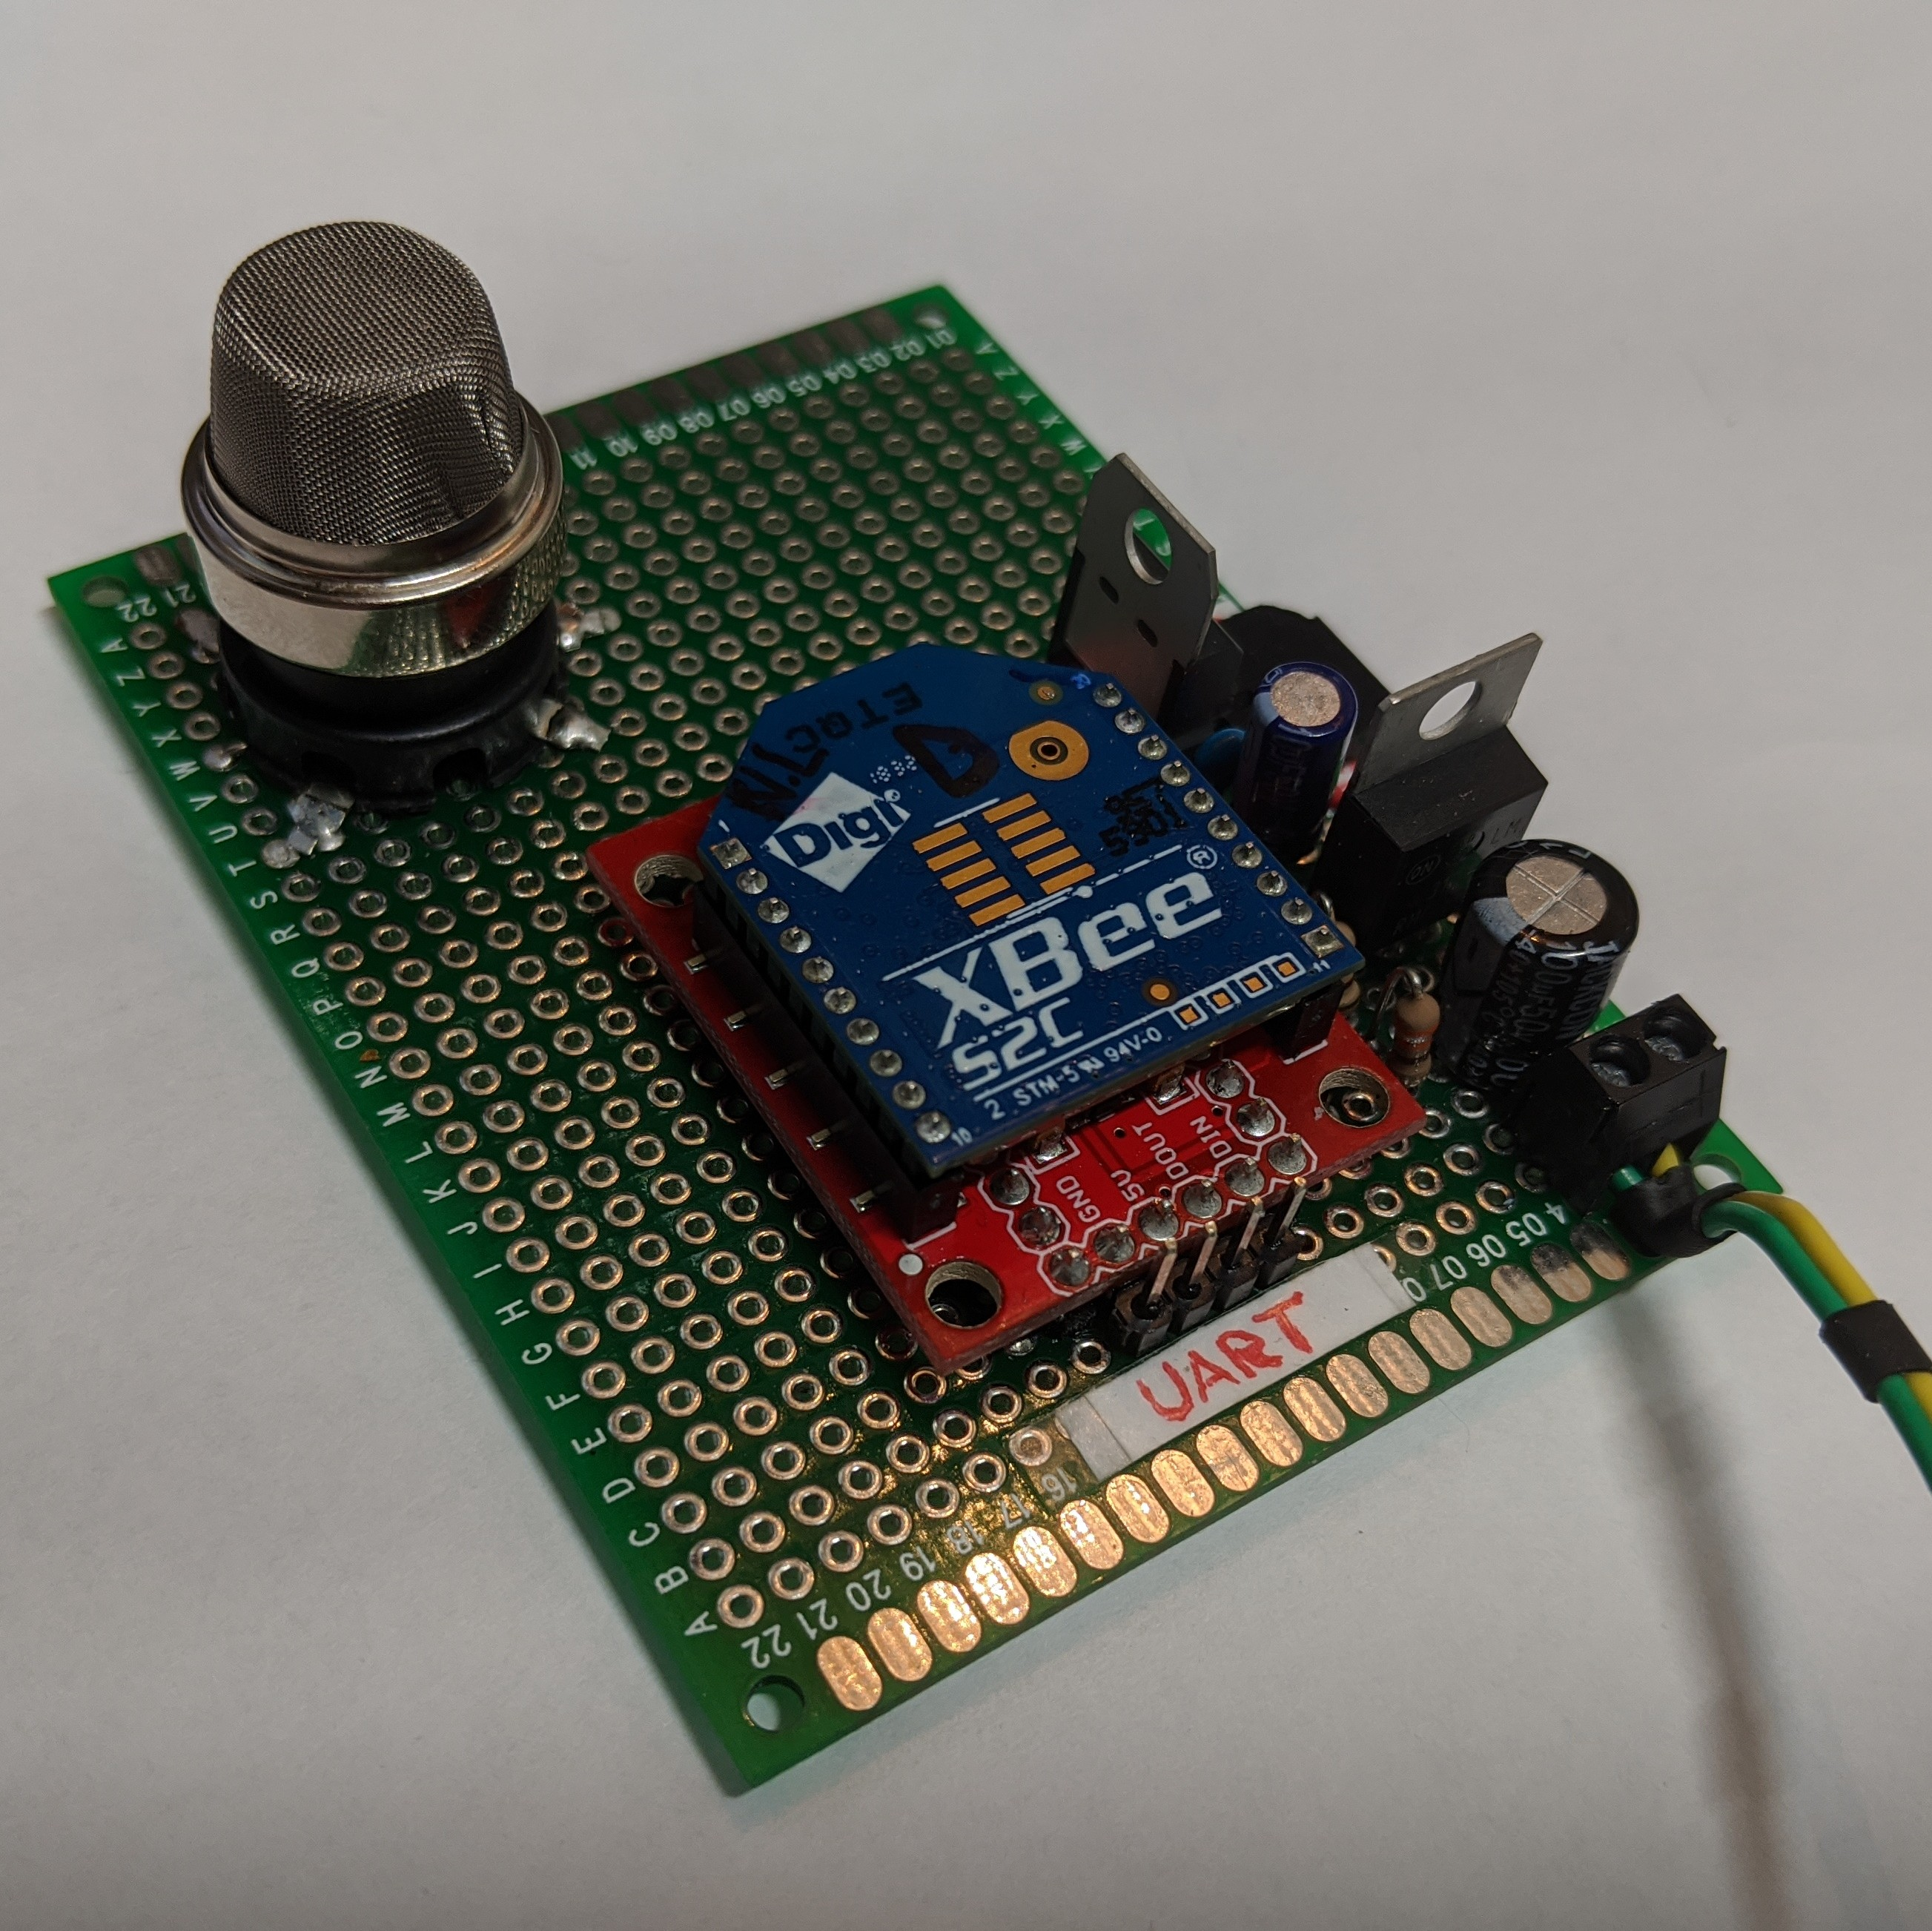
\includegraphics[width=\linewidth]{module_gas.jpg}
			\caption{Gas Module}
		\end{subfigure}
		\begin{subfigure}[t]{0.45\textwidth}
			\centering
			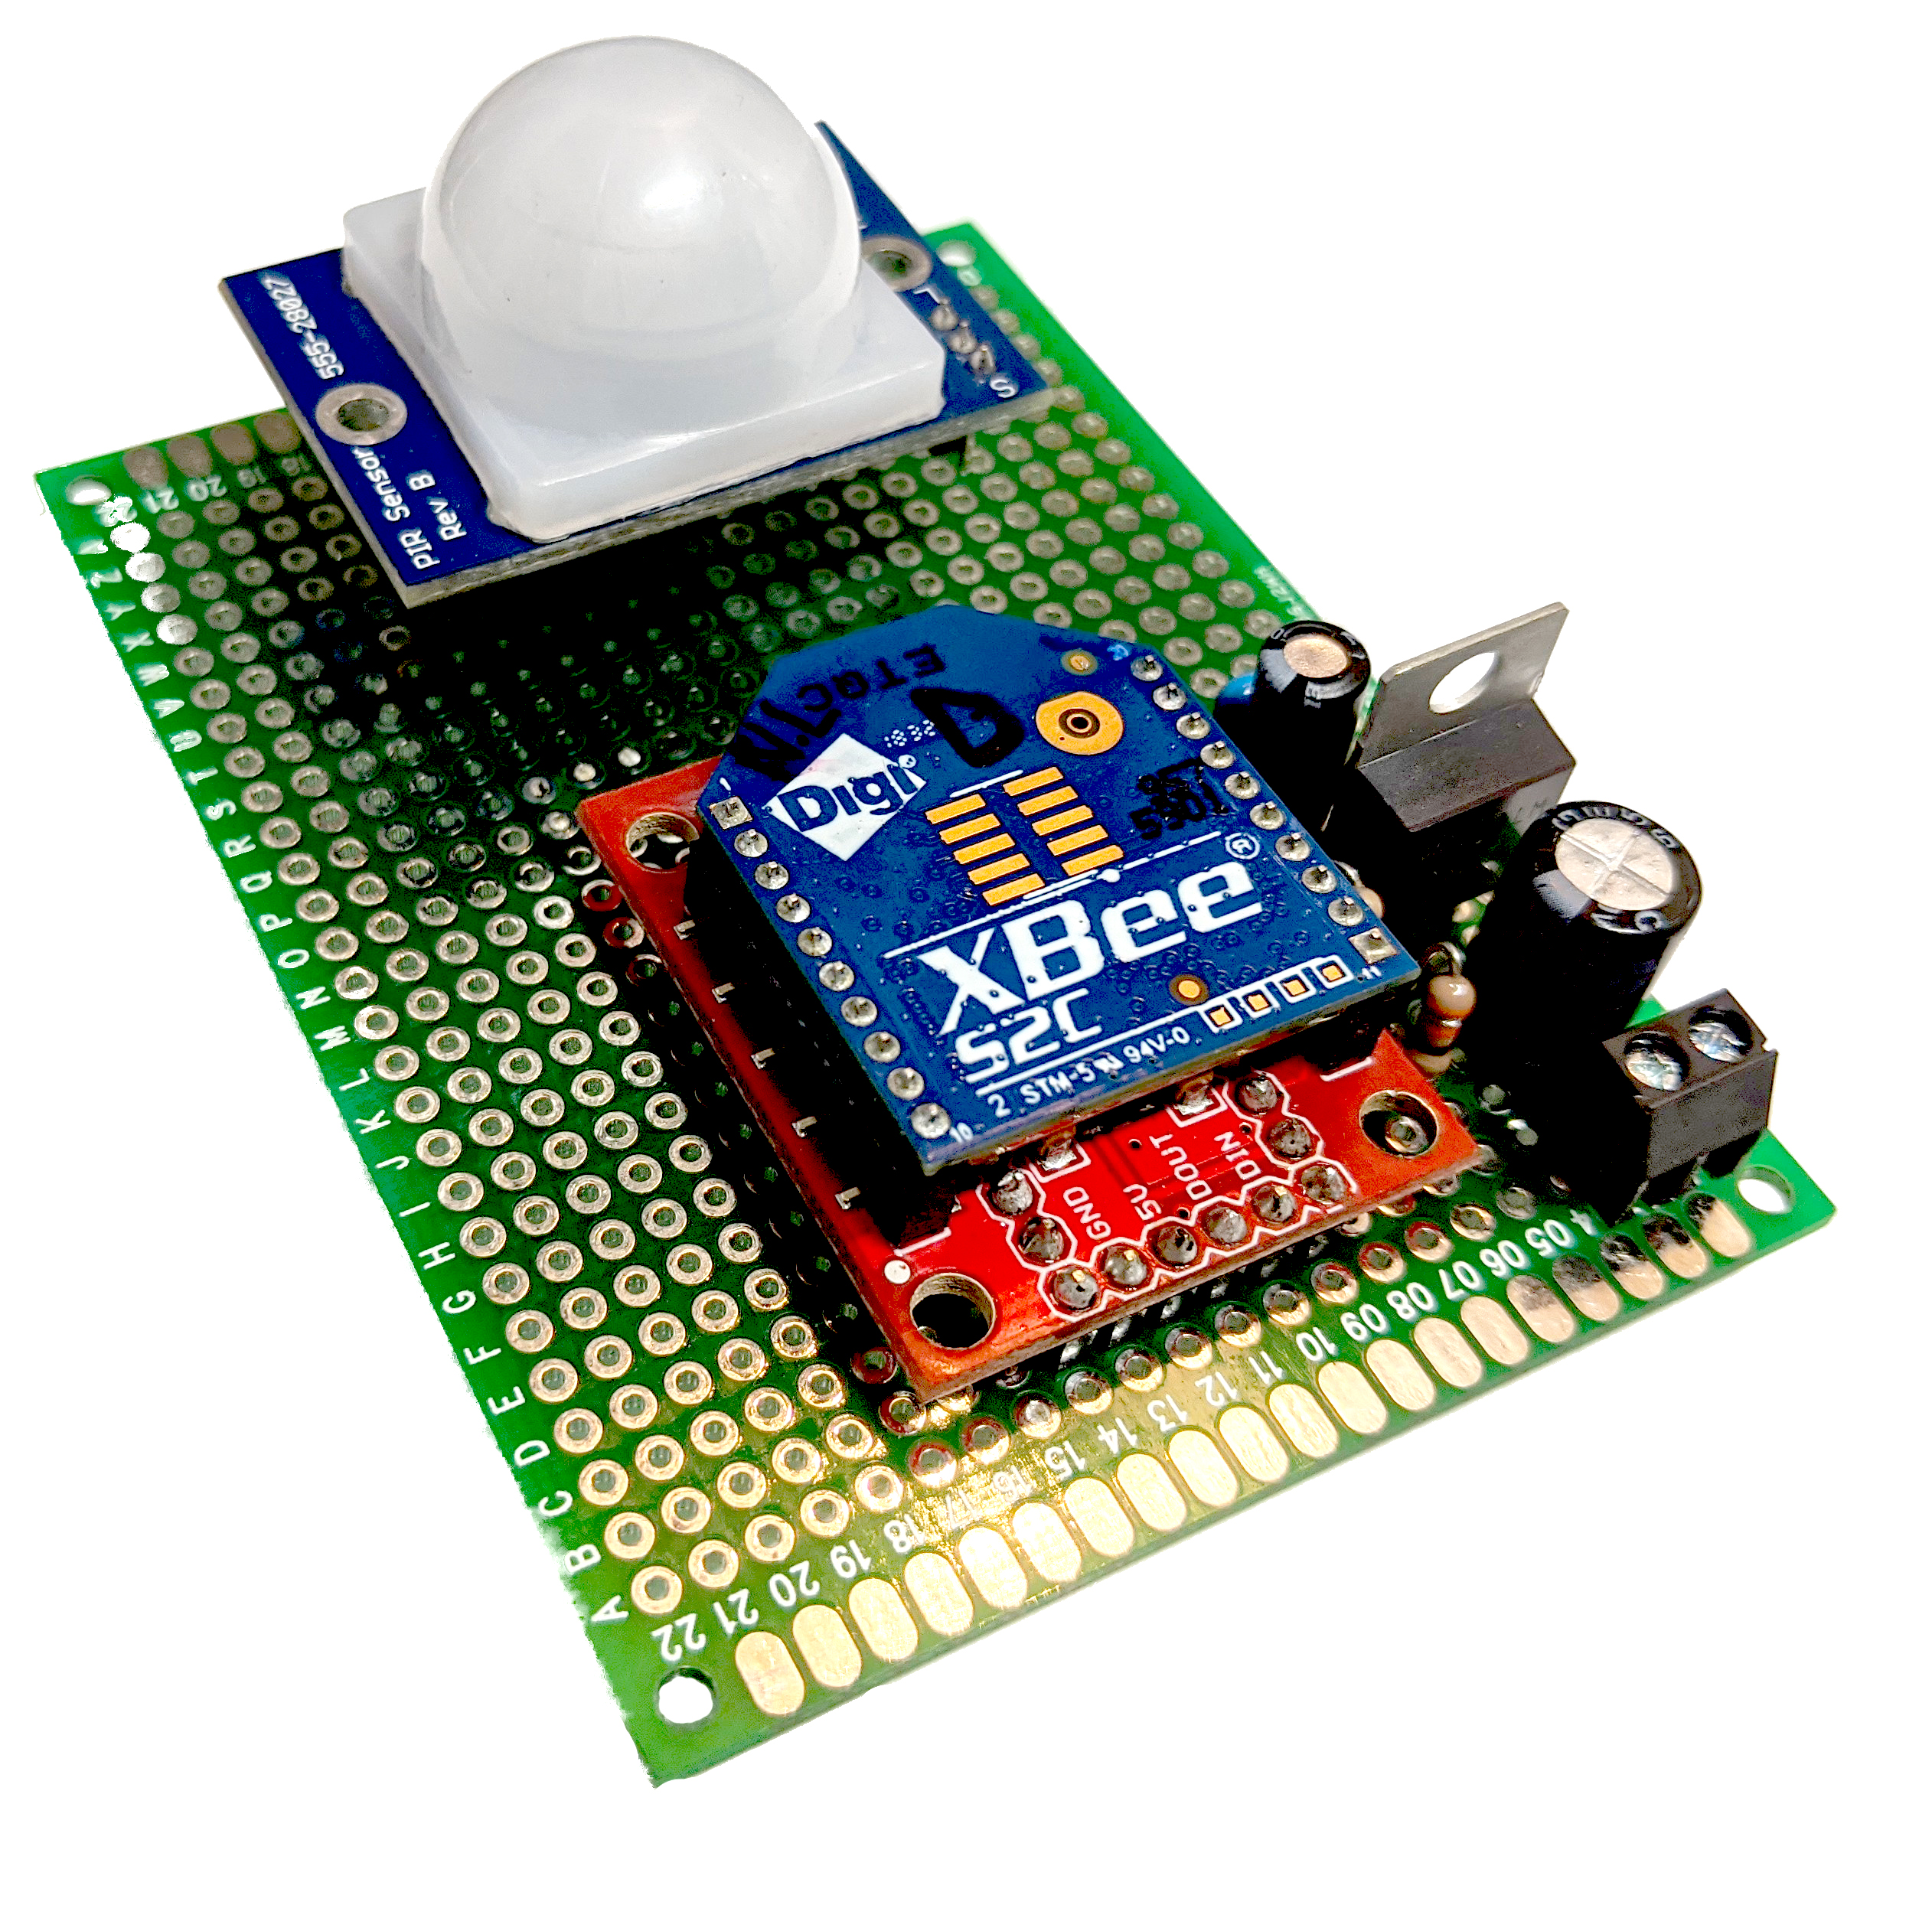
\includegraphics[width=\linewidth]{module_motion.jpg}
			\caption{Motion Module}
		\end{subfigure}
		\caption{Internals of Gas (a), and Motion (b) sensing units}
	\end{figure}
	\par A custom schematic diagram, PCB layout (Figure\ref{fig:pcb}) and 3D model (Figure \ref{fig:3dmodel}) were created to demonstrate the small potential form factor of the units themselves. With surface mount components, including the XBee S2C surface mount model could be used to manufacture extremely effective sensing devices in an incredibly small package.
	\onecolumn
	\begin{figure}[h]
		\centering
		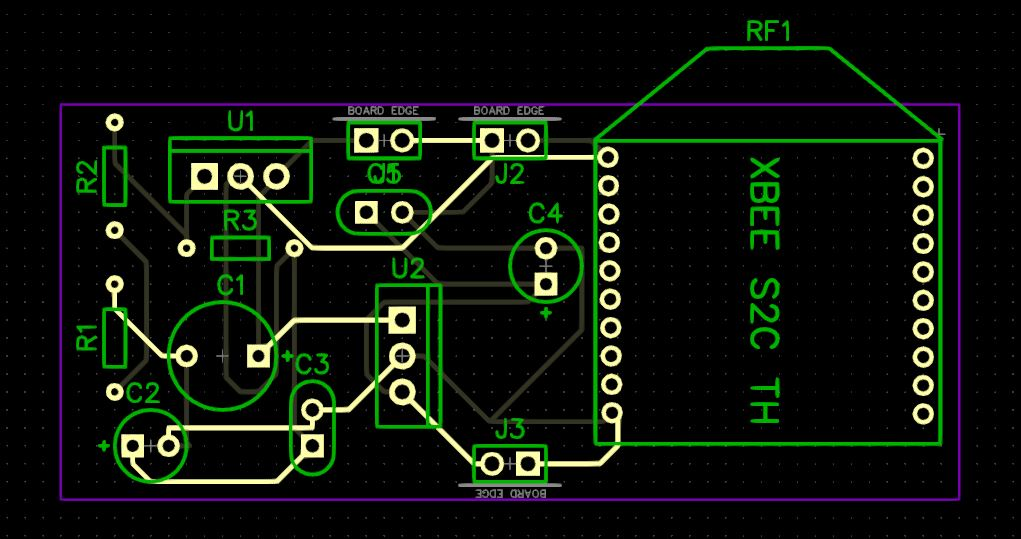
\includegraphics[width=0.75\linewidth]{power supply pcb w xbee.JPG}
		\caption{PCB Layout, 2 layer + top silk screen}
		\label{fig:pcb}
	\end{figure}
	\begin{figure}[h]
	\centering
		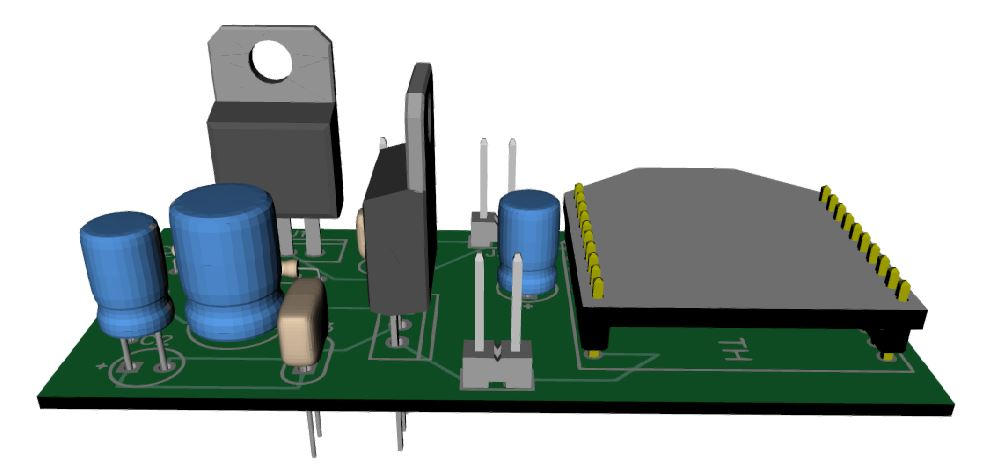
\includegraphics[width=0.75\linewidth]{3dmodel.JPG}
		\caption{CAD Generated 3D Model of PCB including 3.3 \& 5 V power supplies, test points, XBee Module}
		\label{fig:3dmodel}
	\end{figure}
	
	\par Note: The pattern (PCB footprint) of the XBee S2C through-hole model has been designed accurately up to 1 mil (0.001 inches). CAD libraries often do not have the component pattern or schematic of most specialized ICs and other components. If you wish yo use it in a PCB design the schematic, pattern, pin layout/numbering/types, and dimensions must all be measured or documented to a high precision. I used the dimensions found in the technical drawings in the XBee S2C manufacturer data sheet to design the schematic and pattern for the XBee device. 

	\twocolumn
	
	